% BEGIN preamble
\svnidlong
{$HeadURL: file:///mnt/between/svn/dysgu/trunk/DoctoralAcademy/gweithdai-latex/gweithdy-latex-da-2-pellach/training.tex $}
{$LastChangedBy: cfrees $}
{$LastChangedRevision: 10070 $}
{$LastChangedDate: 2024-06-02 15:30:44 +0100 (Sul, 02 Meh 2024) $}

\usepackage[citestyle=authoryear-comp,bibstyle=authoryear,mergedate=basic,isbn=false,url=true,sortcites=true,backend=biber,mincrossrefs=6]{biblatex}
\bibliography{training}

\input{config/macros-da.cfg}

\mode<article>
{
  \usetikzlibrary{quotes,automata,positioning,bending,shadows,shapes.arrows}
  \usepackage{tikz-cd}
}


\title{\LaTeX{} II: Floats, Tips \& Tricks}
\subtitle{Based in part on materials produced by UK-TUG Volunteers}
\date{\cymraeg{Mai} 8 May 2018}

% END preamble

\begin{document}

\begin{frame}
  \titlepage
\end{frame}

\maketitle

\tutornote{Time: 10:00}

\tableofcontents

\mode<presentation>%
{
  \begin{frame}{Outline}
	\tableofcontents
  \end{frame}
}

% Topics covered will include:
%
% Q floating environments – Figures & Tables
% Q tips & tricks

\section{Introduction}

\begin{frame}{\LaTeX{}: Key features}

  \begin{itemize}
	\item \TeX{} is a typesetting application.
	\item \TeX{} uses \emph{primitives} to determine how to put text on a page.
	\item \LaTeX{} is  a \emph{format} built on top of \TeX{}.
	\item \LaTeX{} can be used for everything from a one page letter to a 1000~page textbook.
	\item By separating input from output, reusing material becomes much easier.
	\item By separating \emph{content} from \emph{formatting}, we can create flexible, consistent documents which are easier to maintain and modify.
	\item We are using the \emph{engine} pdf\TeX{}.
	Xe\TeX{} and Lua\TeX{} are modern alternatives.
  \end{itemize}

\end{frame}

\mode<all>
\overleaf
\mode*

\section{Managing floats}\tutornote{10:15}

\begin{frame}[fragile]{Floats}
	You are familiar with floats.
    \begin{columns}[t]
	  \begin{column}{.45\textwidth}
		\begin{semiverbatim}
		  \alert<2>{\\begin\{figure\}[htbp]}
		  \\centering
		  \\includegraphics\{myimage\}
		  \\caption\{A Sample Figure\}
		  \\label\{fig:sample\}
		  \alert<2>{\\end\{figure\}}
		\end{semiverbatim}
	  \end{column}
	  \begin{column}{.45\textwidth}
		\begin{semiverbatim}
		  \alert<2>{\\begin\{table\}[htbp]}
		  \\centering
		  \\caption\{A Sample Table\}
		  \\label\{tab:sample\}
		  \\begin\{tabular\}\{lcr\}
		    a & b & c\\\\
		  \\end\{tabular\}
		  \alert<2>{\\end\{table\}}
		\end{semiverbatim}
	  \end{column}
	\end{columns}
\end{frame}

\begin{frame}{Float control}
  Floats can be tricky to control because they\dots float\dots.
  
  You can influence where they end up in various ways.
  \begin{itemize}
    \item Alter the number or size of floats which \LaTeX{} allows in various places.
    \item Add \texttt{!} to the float specification to ignore those constraints for a particular float.
    \item Issue \cs{clearpage} to force \LaTeX{} to output any floats in the queue.
    \item Move a float a bit earlier or later in the text.
    \item Use package \pkg{placeins} to create \cs{FloatBarrier}s manually or automatically.
  \end{itemize}
  
  \onslide<2->
  If you do not want something to move, however, don't use a float.
  \begin{itemize}
    \item \pkg{capt-of} or \pkg{caption} allow you to use \cs{captionof} for non-floats.
  \end{itemize}
\end{frame}

\begin{exercise}
  \label{ex:floatmanagement}%
  If you have a document with a number of floats, sections etc., you may wish to experiment with that.
  Otherwise, the following example, available at \url{https://www.overleaf.com/read/mnfzhffpzmck} or \url{https://github.com/cfr42/latex-1-2/blob/master/gweithdy-latex-da-2-pellach/examples/example16.tex}, may make a useful starting point.
  \verbatiminput{examples/example16}

  How well does \LaTeX{} do in placing the floats ‘sensibly’?

  Experiment with the effect of different specifications for placement.

  Assuming your document has sections etc., what is the effect of adding \cs{usepackage}\oarg{section}\marg{placeins} to your preamble?

  Try adding an explicit \cs{FloatBarrier} somewhere interesting.
  What difference does this make?

  Suppose that you do not want a particular figure to move.
  Try adding \cs{usepackage}\marg{caption} to your preamble and then add the following somewhere in the middle of your document.
  \begin{verbatim}
    \begin{center}
      \includegraphics{example-image-a}
      \captionof{figure}{A caption for this non-floating figure.}\label{fig:nonfloating}
    \end{center}
  \end{verbatim}
  (You will also need to load \pkg{graphicx} if you are not already doing so).

  What happens to the numbering of figures after the non-floating one?
\end{exercise}

\section{Drawing \& Plotting}\tutornote{11:00}

\begin{frame}{Cautions}
  \begin{itemize}
    \item \TeX{} is Turing complete.
    So, you \emph{can} use it to do all your calculations etc.
  \end{itemize}
  But \dots
  \begin{itemize}
    \item \TeX{} is designed for typesetting.
    \item \TeX{} is \textbf{not} designed to handle complex data manipulation.
  \end{itemize}
\end{frame}
\begin{frame}[fragile]{General advice}
  \begin{itemize}
    \item Use the right tool --- or one of the right tools --- for the job.
    \item If compilation is unbearably slow, you may not be using the best tools.
    \item Use external programmes for complex calculations, filtering of large data sets and manipulation of values.
    \item Use \LaTeX{} packages for simple calculations and manipulations, for presentation and typesetting.
    \item Consider using \verb|gnuplot| etc.\ to calculate plots.
    Use \LaTeX{} with \pgf{} to draw the results.
    \item Consider using \verb|mysql| etc.\ to handle large data sets.
    Use \LaTeX{} with \pkg{datatool} to typeset the results of queries etc.
    \item Use \Tikz{} and \pgfplots{} \pkg{external} libraries and/or \pkg{standalone} when using \TeX{} to draw or plot.
  \end{itemize}
\end{frame}
\begin{frame}[fragile]{Pictures \& Plots}
  \begin{itemize}
    \item \alert<1>{\pgf{}} is a drawing package for \TeX{} with a \LaTeX{} interface.
    \item \alert<1>{\Tikz{}} is a front-end for \pgf{}.
    \item \tikzpgf{} can be used to plot data directly, can integrate \verb|gnuplot| output and can be used to draw diagrams and illustrations of various kinds.
    \onslide<2->
    \item \alert{\pgfplots{}} is a package for drawing plots, based on \tikzpgf{}.
    \item \alert{\pgfplotstable{}} is a package provided by \pgfplots{} for constructing tables from data.
  \end{itemize}
\end{frame}

\subsection{Drawing}

\begin{frame}[fragile]{Diagrams}{A Simple \Tikz{} Picture}
  \begin{columns}
    \begin{column}{.75\linewidth}
\begin{semiverbatim}
\\documentclass\{standalone\}
\alert<1>{\\usepackage\{tikz\}}
\\begin\{document\}
\alert<2>{\\begin\{tikzpicture\}}
\alert<3>{\\path [fill=gray, draw=darkgray] 
  (0,0) -{}- (1,1) arc (45:0:1) -{}- cycle;}
\alert<2>{\\end\{tikzpicture\}}
\\end\{document\}
\end{semiverbatim}
    \end{column}%
    \begin{column}{.25\linewidth}
      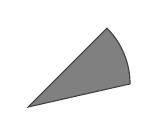
\begin{tikzpicture}
    \path [fill=gray, draw=darkgray] (0,0) -- (1,1) arc (45:0:1) -- cycle;
  \end{tikzpicture}
    \end{column}
  \end{columns}
\end{frame}
\begin{frame}<1-| article:0>[fragile,plain]%{Another Simple(-ish) \Tikz{} Picture}
   \begin{columns}
    \begin{column}{.75\linewidth}
\begin{semiverbatim}
\\begin\{tikzpicture\}[line width=.5pt]
  \\shade [draw=blue!50!cyan!75!black, line width=.5pt, 
  double distance=.25pt, double=blue!50!cyan!50!white, 
  inner color=blue!50!cyan!25!white, outer 
  color=blue!50!cyan!75!black, opacity=1, draw opacity=1] 
  (0,0) circle (1.425);
  \\begin\{scope\}[blend mode=screen, opacity=.5]
    \\clip (0,0) circle (1.415);
    \alert{\\foreach \\k} [count=\\c, evaluate=\\c as 
    \\f using \{\\c*100/7\}] in 
    \{0,2.5,5,...,12.5\}
    \{\\begin\{scope\}[rotate=\alert{\\k}]
      \alert{\\foreach \\j} in \{0,15,30\}
        \{\\scoped[rotate=\alert{\\j}]\{\\draw [blue!\\f!green] \alert{\\foreach 
          \\i} in \{0,45,...,315\} \{ (\alert{\\i}:1) circle (1) \};\} \}
      \\end\{scope\} \}
  \\end\{scope\}
\\end\{tikzpicture\}
\end{semiverbatim}
    \end{column}
    \begin{column}{.25\linewidth}
      \vspace*{2\baselineskip}
      \includegraphics{examples/tikz-siml}
    \end{column}
  \end{columns}
\end{frame}
% do NOT comment end of line above!!
Another still simplish \Tikz{} picture demonstrates the use of \verb|\foreach| loops to construct pictures with patterned elements\footnote{\url{https://github.com/cfr42/latex-1-2/blob/master/gweithdy-latex-da-2-pellach/examples/tikz-siml.tex}} (\cref{fig:tikz-siml}):
\begin{figure}
  \centering
  \documentclass[11pt]{standalone}
\usepackage{tikz}
\begin{document}
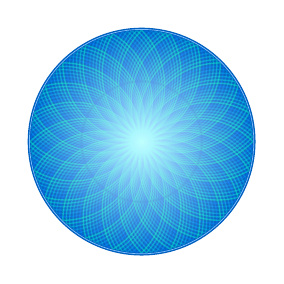
\begin{tikzpicture}[line width=.5pt]
  \shade [draw=blue!50!cyan!75!black, line width=.5pt, double distance=.25pt, 
  double=blue!50!cyan!50!white, inner color=blue!50!cyan!25!white,
  outer color=blue!50!cyan!75!black, opacity=1, draw opacity=1] (0,0) circle (1.425);
  \begin{scope}[blend mode=screen, opacity=.5]
    \clip (0,0) circle (1.415);
    \foreach \k [count=\c, evaluate=\c as \f using {\c*100/7}] in {0,2.5,5,...,12.5}
    {\begin{scope}[rotate=\k]
        \foreach \j in {0,15,30}
        {
          \scoped[rotate=\j]{
            \draw [blue!\f!green] \foreach \i in {0,45,...,315} { (\i:1) circle (1) };
          }
        }
      \end{scope}
    }
  \end{scope}
\end{tikzpicture}
\end{document}

  \caption{Output from \textt{tikz-siml.tex}.}\label{fig:tikz-siml}
\end{figure}
\verbatiminput{examples/tikz-siml}%




\subsection{Handling Data}

\begin{frame}[fragile]{\texttt{pgfplotsexample.tex}}
  The handout includes a copy of \texttt{pgfplotsexample.tex}\only<0| handout:1>{\footnote{\url{http://mirrors.ctan.org/graphics/pgf/contrib/pgfplots/doc/pgfplotsexample.tex}}}
  \begin{semiverbatim}
    \\usepackage\{pgfplots\}
    \alert<2>{\\pgfplotsset\{compat=1.8\}}
  \end{semiverbatim}
  \onslide<2->
  The \verb|compat| setting determines which features are available (and which bug fixes).

  Use \verb|newest| for the latest and greatest.
%
  Use the current version number for the latest and greatest, ensuring your code will produce the same results with newer versions.
\end{frame}

\verbatiminput{examples/pgfplotsexample}

\begin{frame}[fragile]{\texttt{pgfplotsexample.tex}}
  \begin{semiverbatim}
    \alert<2>{\\begin\{tikzpicture\}}
      \alert<3>{\\begin\{loglogaxis\}}
        \alert<4>{\\addplot} \alert<5>{coordinates} \alert<6>{\{
          (1,1)
          (16,16)
          (32,64)
        \}}\alert<7>{;}
      \alert<3>{\\end\{loglogaxis\}}
    \alert<2>{\\end\{tikzpicture\}}
  \end{semiverbatim}
\end{frame}

\begin{frame}[fragile]{Tables of Data}
  \pgfplots{} can also plot from a \verb|table| of data.

  The table may be specified either inline or in an external file.

  \cs{addplot} \alert<2,6>{\texttt{table}} \alert<3,7-9>{\oarg{column selection}} \alert<4,10>{\marg{file or inline table}}\texttt{;}

  \onslide<6->
  An example data file, \alert<10>{\texttt{datafile.dat}}, from the manual (p.~47) is included in the handout.

  \begin{semiverbatim}
    \\addplot \alert<6>{table} \alert<7>{[}\alert<7,8>{x=dof}\alert<7>{,}\alert<7,9>{y=L2}\alert<7>{]} \alert<10>{\{datafile.dat\}};
  \end{semiverbatim}

\end{frame}

\verbatiminput{examples/datafile.dat}

\begin{exercise}
  Try creating some plots with \cs{addplot} \texttt{coordinates}.

  Now create a simple data file and experiment with the \texttt{table} function.

  The \env{loglogaxis} environment takes an optional argument which can be used to specify the appearance of the axes and plot in key-value format.
  What does adding \textt{xlabel=my label,ylabel=your label} as an optional argument do?
\end{exercise}

\mode<all>
\furtherinfo*[%
  Appendix \ref{handouts:sec:fff}: descriptions of, and pointers to, the following float-related resources.
  \begin{itemize}
    \item \citetitle{mittelbach-hipfeftl} \autocite{mittelbach-hipfeftl}.
    \item Manuals for \pkg{placeins}, \pkg{float} and \pkg{endfloat}.
  \end{itemize}
  \item Appendix \ref{handouts:sec:samples}: sample output for exercise \ref{handouts:ex:floatmanagement} and \texttt{pgfplotsexample.tex}.
  \item Appendix \ref{handouts:sec:fn}: example illustrating the use of \pgfplots{} to plot a function.
  \item Appendix \ref{handouts:sec:dpr}: further resources for plots and diagrams.
]
\mode*


% \clearpage
\appendix


\section<1-| beamer:0>{Further Float Fun}\label{sec:fff}
% BEGIN sec:fff

\begin{itemize}
  \item \fullcite{mittelbach-hipfeftl}.
  Authoritative article describing the way in which \LaTeX{} places floating material and the builtin features which can be used to influence the results.
  This text does not cover packages available to extend the facilities provided by the \LaTeX{} kernel.
  Copies are included among the workshop handouts.
  \item \pkg{placeins}'s manual: \url{http://mirrors.ctan.org/macros/latex/contrib/placeins/placeins-doc.pdf}.
  Insert \cs{FloatBarrier}s to corral floats into particular parts of a document, or automatically constrain floats to the sections of a document in which they are defined.
  \item \pkg{float}'s manual: \url{http://mirrors.ctan.org/macros/latex/contrib/float/float.pdf}.
  Interface for defining new types of floats and customising the typesetting of existing ones.
  The \verb|H| placement specifier is widely abused.
  Do not use this simply because you don't want a float to float.
  Use a non-float, with \cs{captionof}, if you want a caption.
  Treat \verb|H| as a strategy of last resort which \emph{may} be useful if you have complex customised formatting for floats which you want to apply to a non-float.
  Using it merely in order to use \cs{caption} invites trouble to tea.
  \item \pkg{endfloat}'s manual: \url{http://mirrors.ctan.org/macros/latex/contrib/endfloat/endfloat.pdf}.
  Move all floats to the end of the document, optionally inserting markers into the document when the floats are defined.
  Some journals require this.
\end{itemize}

% END sec:fff

\section<1-| beamer:0>{Sample Output}\label{sec:samples}
% BEGIN sec:samples

\subsection<1-| beamer:0>{Float Examples}\label{subsec:samples-floats}
% BEGIN subsec:samples-floats
This appendix includes sample output for the code in \cref{ex:floatmanagement}.

The output of the original code is shown first\footnote{\url{https://github.com/cfr42/latex-1-2/blob/master/gweithdy-latex-da-2-pellach/examples/example16.tex}}.

This is followed by the result when \cs{usepackage}\oarg{section}\marg{placeins} is added to the preamble\footnote{\url{https://github.com/cfr42/latex-1-2/blob/master/gweithdy-latex-da-2-pellach/examples/example16-mod.tex}}.
\includepdf{examples/example16}
\includepdf{examples/example16-mod}
% END subsec:samples-floats

\subsection<1-| beamer:0>{Plot Examples}\label{subsec:samples-plots}
% BEGIN subsec:samples-plots
\Cref{fig:pgfplotsexample} shows sample output from the \pgfplots{} example \textt{pgfplotsexample.tex}.
Output from the plot in \cref{sec:fn} is included later in \cref{fig:sin}.
\begin{figure}
  \centering\includegraphics[width=\textwidth]{examples/pgfplotsexample}
  \caption{Output for \textt{pgfplotsexample.tex}.}\label{fig:pgfplotsexample}
\end{figure}
% END subsec:samples-plots

% END sec:samples

\section<1-| beamer:0>{Plotting Functions}\label{sec:fn}
% BEGIN sec:fn

This appendix illustrates how to plot a function using \pgfplots.
\Cref{fig:sin} shows sample output from the code listing\footnote{\url{https://github.com/cfr42/latex-1-2/blob/master/gweithdy-latex-da-2-pellach/examples/pgfplots-sin.tex}}.

\verbatiminput{examples/pgfplots-sin}
\begin{figure}
  \centering
  \includegraphics{examples/pgfplots-sin}
  \caption{$\sin$ function, plotted with \protect\pgfplots.}\label{fig:sin}
\end{figure}
% END sec:fn

\section<1-| beamer:0>{Drawing Diagrams}\label{sec:dd}
% BEGIN sec:dd

\Tikz{} can do an impressive amount, even when it is not the most efficient tool for the job.
This appendix includes a few of the more basic examples, but be aware that if your project needs ducks, nuns or snow persons, you will find others have already addressed your need in the form of third-party packages and libraries.
Syntactic trees, circuit diagrams, lattices, knots and improved  curves may be designed for less seriously minded users, but could nonetheless brighten up your day.

\foreach \i in {tikz-annotated-cuboid,tikz-automata-finite-state-transducer,tikz-ticking-timers,tikz-cd-eg,tikz-shaded-delaunay-pattern} {%
  \begin{figure}
    \centering
    \input{examples/\i}
    \caption{\url{github.com/cfr42/latex-1-2/blob/master/gweithdy-latex-da-2-pellach/examples/\i.tex}}
  \end{figure}
}

% END sec:dd

\section<1-| beamer:0>{Diagram and Plot Resources}\label{sec:dpr}
% BEGIN sec:dpr

\begin{itemize}
  \item \url{www.texample.net} provides a variety of example plots and diagrams organised by programming feature, content, package etc\@.
  The code here is not always current, but the examples do a good job of indicating some of what is possible with \tikzpgf{} and \pgfplots.
  \item \url{tex.stackexchange.com} attracts a lot of questions concerning diagrams and plots.
  Search or sort by relevant tags to find relevant examples.
\end{itemize}

% END sec:dpr

\end{document}
